\begin{figure}[p]
\centering
\captionsetup{justification=raggedright,labelsep=none,singlelinecheck=false,labelformat=boldlabel}
\caption[]{\footnotesize \textbf{: Cross-sectional distribution of net Sharpe ratios for volatility-managed factor portfolios by Jensen, Kelly, and Pedersen factor cluster.} Each box summarizes the factor-level Sharpe ratios within the indicated cluster. The center line is the median, the box spans the interquartile range, and the whiskers extend to the most extreme observations within 1.5 interquartile ranges. Managed strategies cap exposure at 1.5 and deduct 10 basis points per unit change in factor exposure.}
\label{fig:rv-portfolio_cluster_sharpe}
\par\smallskip\textbf{Panel A. Long sample}\par\smallskip
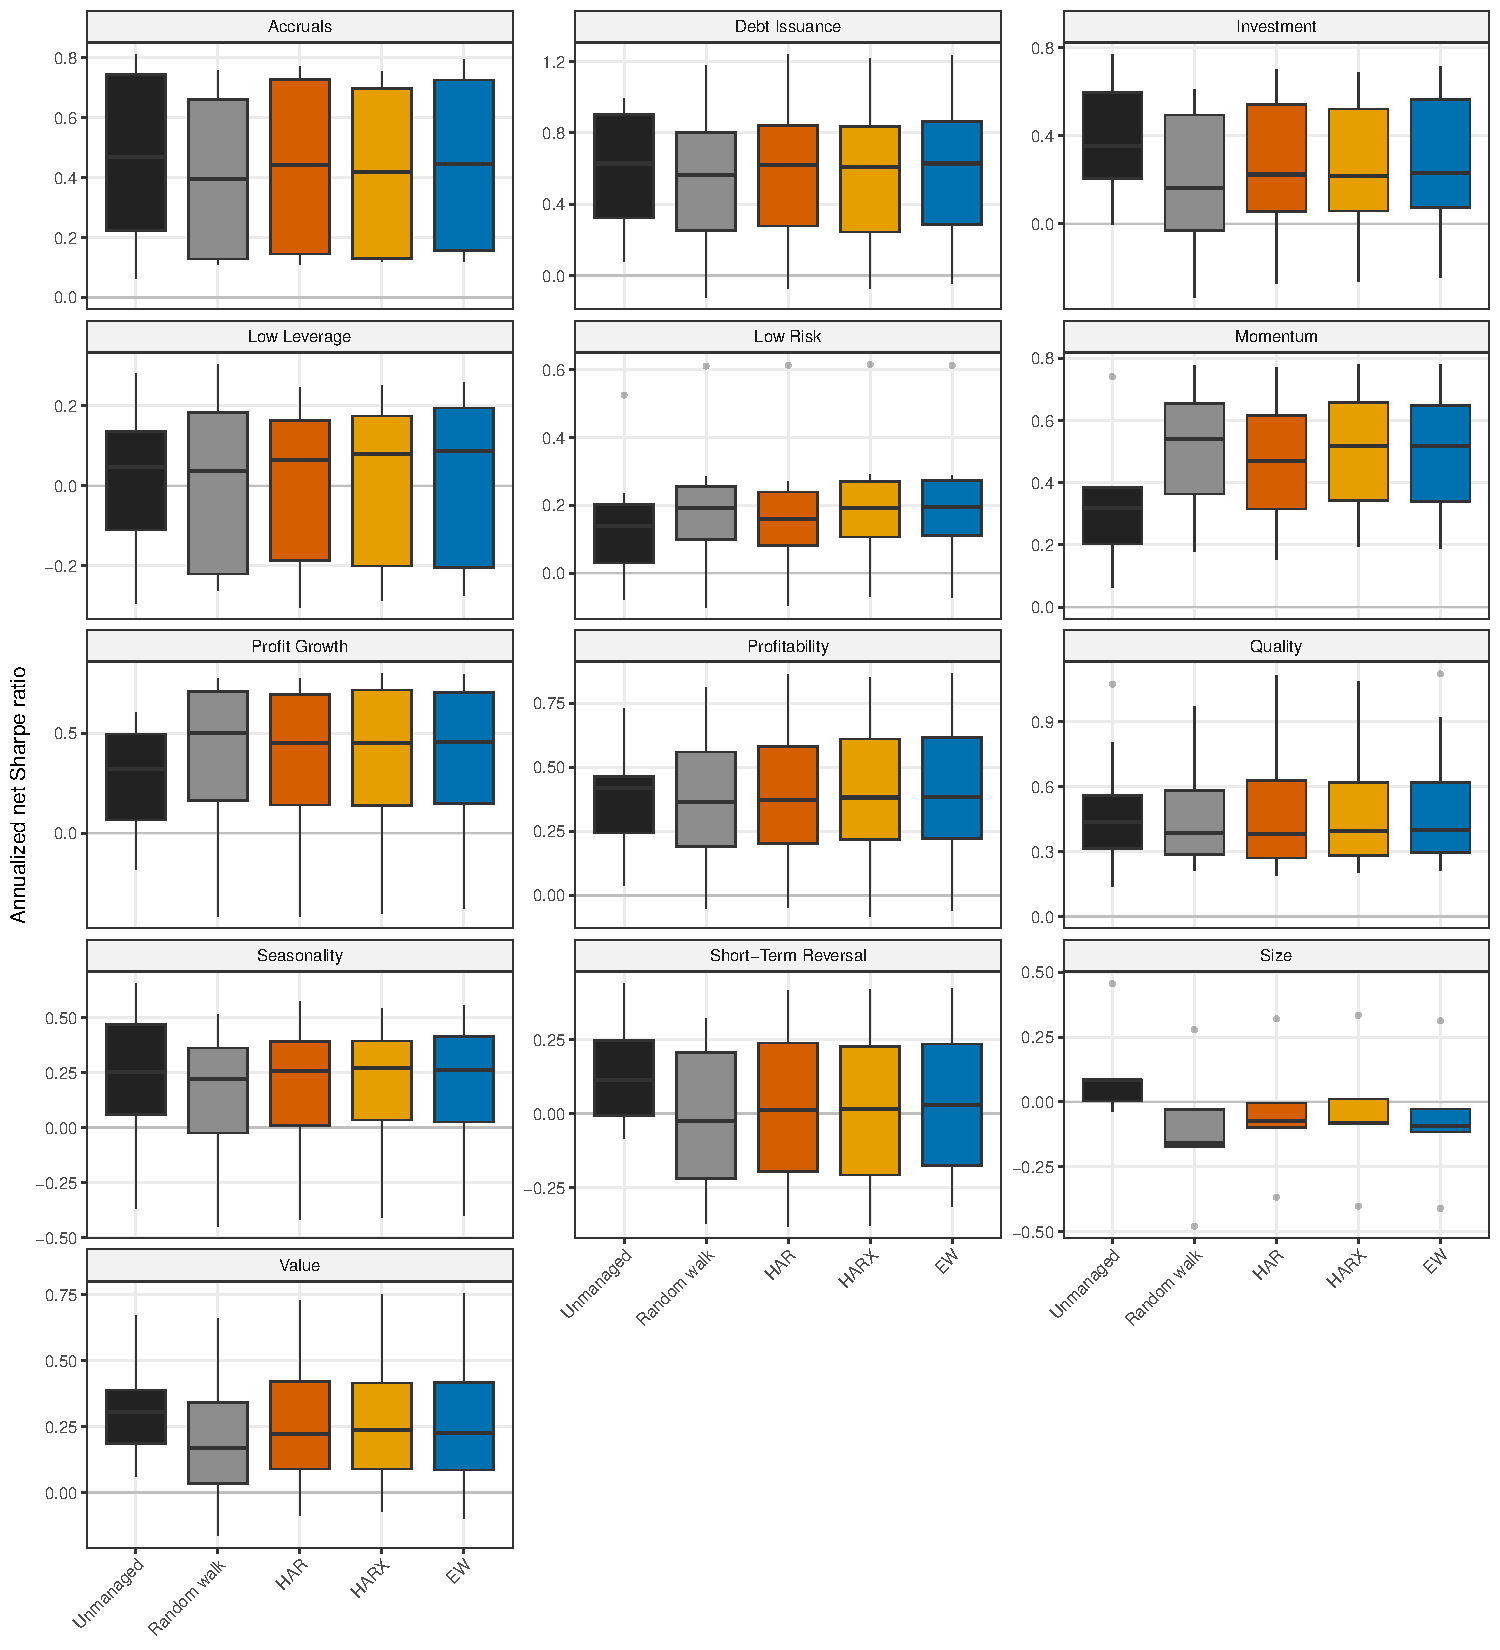
\includegraphics[width=\linewidth,height=0.70\textheight,keepaspectratio]{results_v3/1927/main_appendix/portfolio_cluster_sharpe.pdf}
\end{figure}
\begin{figure}[p]
\ContinuedFloat
\centering
\captionsetup{justification=raggedright,labelsep=none,singlelinecheck=false,labelformat=boldlabel}
\caption[]{\footnotesize \textbf{: Cross-sectional distribution of net Sharpe ratios for volatility-managed factor portfolios by Jensen, Kelly, and Pedersen factor cluster.} Each box summarizes the factor-level Sharpe ratios within the indicated cluster. The center line is the median, the box spans the interquartile range, and the whiskers extend to the most extreme observations within 1.5 interquartile ranges. Managed strategies cap exposure at 1.5 and deduct 10 basis points per unit change in factor exposure. Continued.}
\par\smallskip\textbf{Panel B. Short sample}\par\smallskip
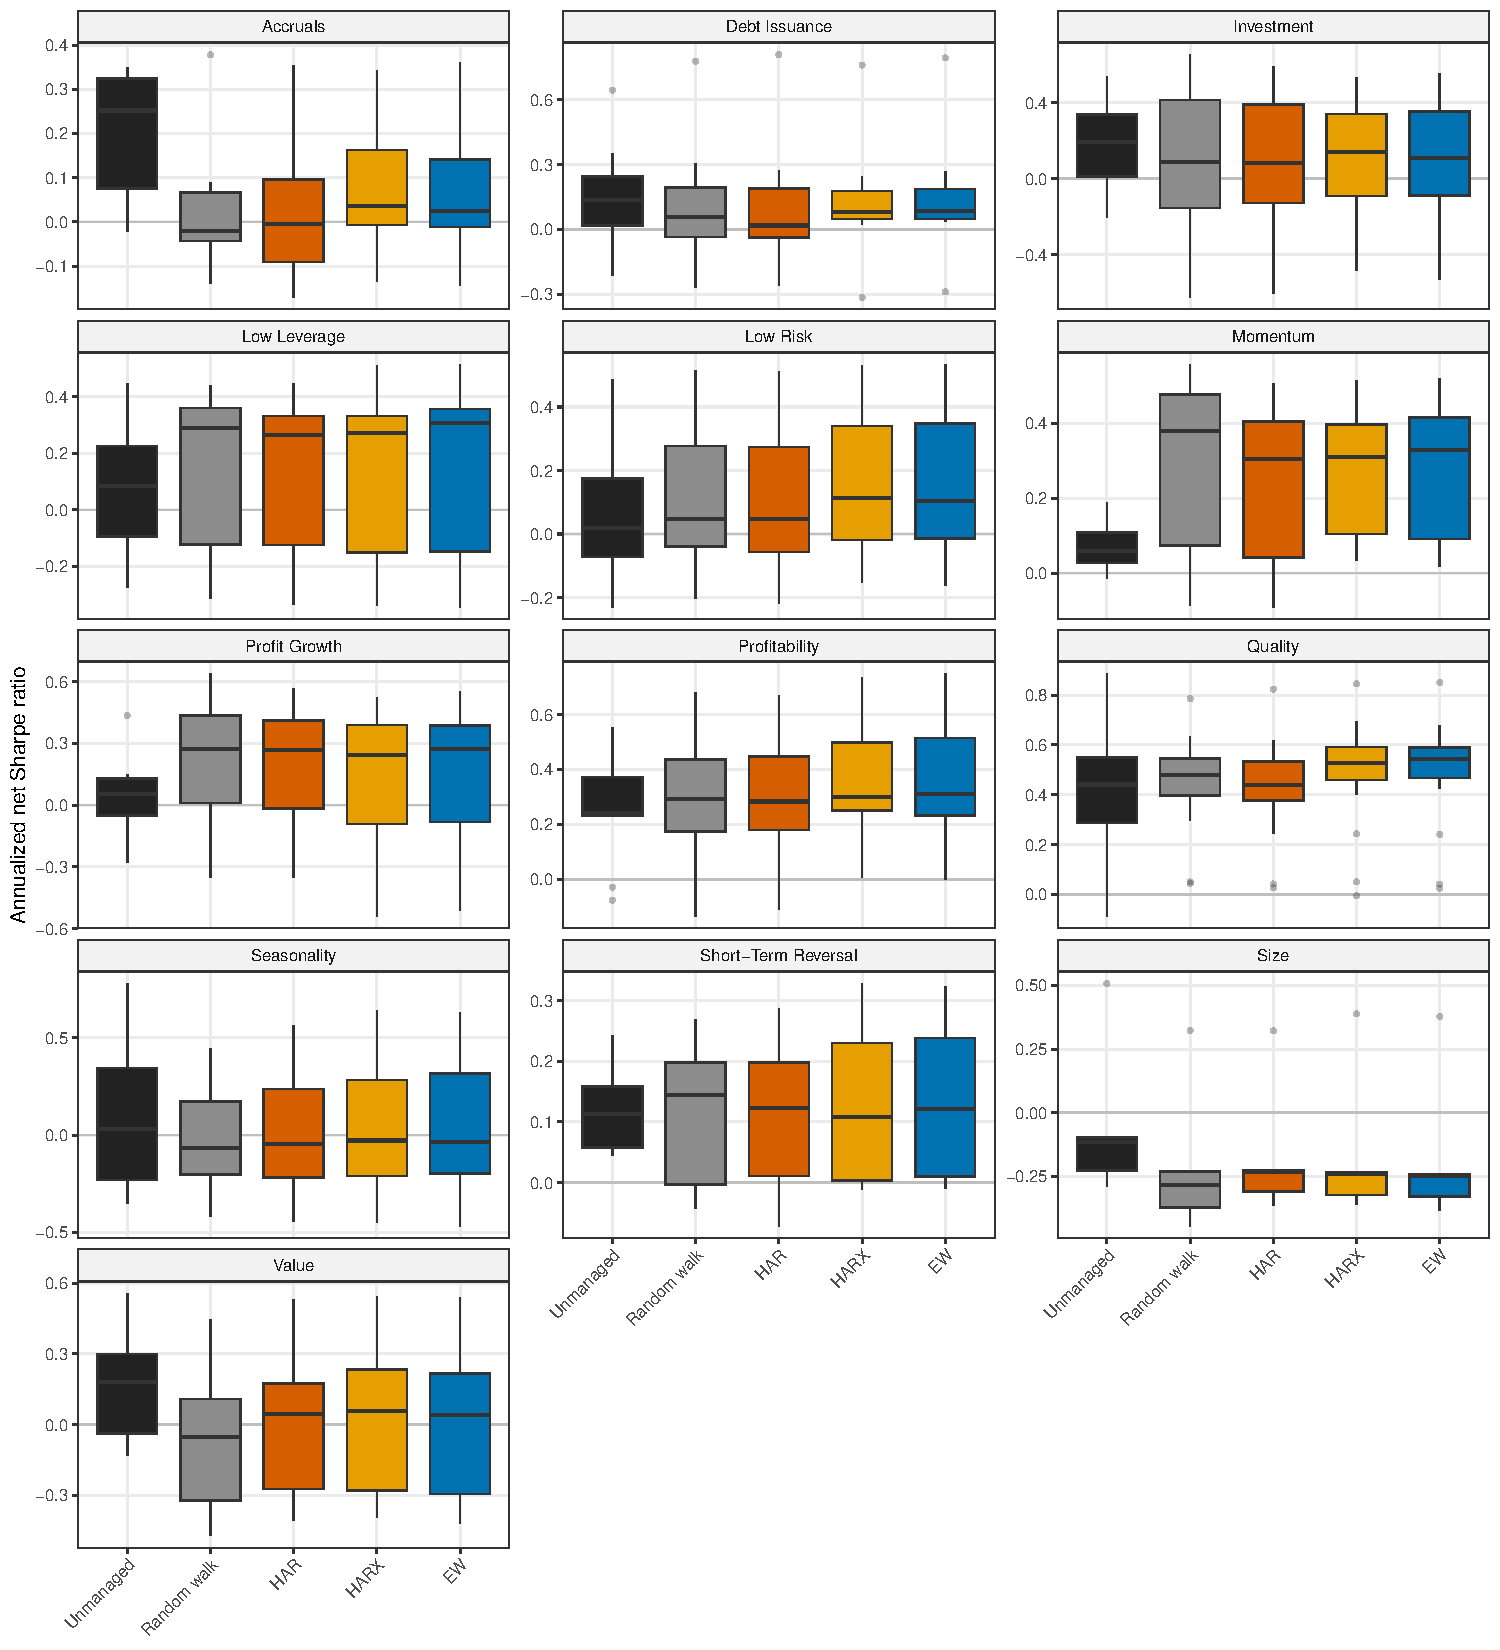
\includegraphics[width=\linewidth,height=0.70\textheight,keepaspectratio]{results_v3/1986/main_appendix/portfolio_cluster_sharpe.pdf}
\end{figure}
